\chapter{Unification of \texorpdfstring{$\lambda$}{λ}-terms and higher-order patterns}\label{ch:hounif}

% ============================================================================================
\section{What this chapter is about}\label{sec:hounif-intro}

The previous chapters built programs whose execution keeps asking one question: \emph{find values for the
logic variables that make two $\lambda$-terms equal modulo $\alpha$, $\beta$ and $\eta$}. \Cref{ch:lambda} showed
how such questions are written as quantified formulas; \cref{ch:hoprog,ch:lambdatree} produced them by the
thousand, from higher-order predicates such as \lp{mappred} and from the \lp{pi x\ ...} goals that walk under
binders in $\lambda$-tree syntax. \Cref{ch:lambdatree} also isolated the fragment $\Llam$, in which a logic
variable is applied only to distinct bound variables. This chapter, which follows Chapter~8 of the
book~\cite{MillerNadathur2012}, explains how an implementation \emph{solves} these questions, and why $\Llam$ is
the fragment to aim for.

The story has two halves.
\begin{enumerate}[nosep]
  \item \textbf{General higher-order unification} is hard: there may be no most general unifier, complete sets
    of unifiers may be infinite, and unifiability is undecidable (\cref{sec:hounif-hard}). Still, Huet's
    procedure~\cite{Huet1975} organises the search (\cref{sec:hounif-huet}): it simplifies rigid-rigid
    equations, \emph{guesses} imitation or projection substitutions for flexible-rigid ones, and stops when only
    flexible-flexible equations are left. Its search space is a \emph{matching tree}, which can be infinite.
  \item \textbf{Higher-order pattern unification} ($\Llam$-unification, \cref{sec:hounif-llambda,sec:hounif-algo})
    is the same procedure restricted to patterns. There it becomes \emph{deterministic}, has \emph{most general
    unifiers} and, with an occurs-check, \emph{terminates}~\cite{Miller1991}. Its final form, \emph{variable
    elimination}, is \enquote{computationally similar to first-order unification} \book{224}: one walk over the
    rigid side that inverts it, prunes, and checks occurrences and scope.
\end{enumerate}
We then do the algorithm by hand on the book's examples (\cref{sec:hounif-traces}), rebuild Nipkow's de~Bruijn
implementation~\cite{Nipkow1993} and run a Scheme transliteration of it (\cref{sec:hounif-nipkow}), and finish
with what real systems do: universe levels instead of raising, and delayed non-pattern equations
(\cref{sec:hounif-pragmatics}). If you only need the implementer's digest, read
\cref{def:hounif-elim,thm:hounif-mgu} and \cref{sec:hounif-nipkow,sec:hounif-pragmatics}.

\paragraph{Conventions.} As in the book's Chapter~8, uppercase $F,G,H,U,V,W,X,Y$ are \emph{existentially}
quantified variables (logic variables), and lowercase $a,b,c,d,f,g,u,w,x,y,z$ are \emph{universally}
quantified ones (signature constants or eigenvariables). $\bar x$ abbreviates $x_1\dots x_n$, and $(F\,\bar x)$
is $(F\,x_1\dots x_n)$.

% ============================================================================================
\section{Unification problems and their normal form}\label{sec:hounif-problems}

\begin{definition}[Unification problem {\book{211}}]\label{def:hounif-problem}
A \emph{unification problem} is a formula
\[
  Q_1x_1\dots Q_nx_n\,[\,t_1=s_1\wedge\dots\wedge t_m=s_m\,]
\]
where $n,m\ge 0$, each $Q_i$ is $\forall$ or $\exists$, and $t_j$, $s_j$ are $\lambda$-terms of the same type. The
quantifier sequence is the \emph{prefix}, the conjunction is the \emph{matrix}. A \emph{unifier} is a substitution
for the existentially quantified variables that makes every $t_j$ $\lambda$-convertible to $s_j$.
\end{definition}

Reading the problem as a formula is what makes the scoping right. In $\exists X\,\forall y\,[X=y]$ no unifier
exists, because $X$ is chosen before $y$ and cannot mention it; in $\forall y\,\exists X\,[X=y]$ the unifier is
$X:=y$. A miniKanren with only first-order terms never sees the difference because it has no universal
quantifier in goals; a $\lambda$Prolog with \lp{pi} sees it all the time.

\Cref{ch:lambda} distinguished a unifier from a \emph{solution}, which in addition uses only closed terms and
therefore \enquote{embodies an actual proof of the quantified formula}; following common practice the book's
Chapter~8 limits itself to unifiers \book{211}. (The difference matters with empty types; see the last pitfall of
\cref{sec:hounif-dynamic}.)

\subsection{The normal form assumed by the algorithms}

Before solving, the book puts every problem in a fixed shape \book{212}. The four steps are worth knowing one by
one, because an implementation performs each of them lazily.
\begin{enumerate}
  \item \textbf{A $\forall\exists\forall$ prefix.} Using \emph{raising} \book{107--108}, the formulas
    $\forall y\,\exists x\,G$ and $\exists h\,\forall y\,G[(h\,y)/x]$ are equiprovable when $h:\sigma\to\tau$ for
    $y:\sigma$, $x:\tau$. Moving every $\exists$ to the left of every $\forall$ in this way yields a prefix
    $\forall\bar a\;\exists\bar X\;\forall\bar y$. The outer $\forall\bar a$ represent \enquote{the ambient signature
    comprising the declared constants in a $\lambda$Prolog program, and we will interpret them as such}
    \book{212}. The price: \enquote{the type of the variable that is existentially quantified needs to be
    \enquote{raised} by the type of the universally quantified variable} \book{108}.
  \item \textbf{Substitution as $\beta$-redex.} For $\theta=\{\langle x_1,t_1\rangle,\dots,\langle x_n,t_n\rangle\}$,
    the book defines \book{212}
    \[\theta(t):=((\lambda x_1\dots\lambda x_n\,t)\,t_1\dots t_n).\]
    Thus $\theta(t)$ and
    $\theta(t')$ are equal whenever $t$ and $t'$ are $\lambda$-convertible, and we may assume all terms are in
    $\beta$-normal form.
  \item \textbf{Equal binders.} By $\eta$-conversion the two sides of every equation get binders of the same
    length.
  \item \textbf{Binders become universals.} Using $(\lambda x\,t=\lambda x\,s)\equiv\forall x\,(t=s)$ and moving
    such $\forall x$ out of the conjunction, the binders at the heads of the equations turn into universals that
    \emph{extend the inner block}. After this step \enquote{the equations in the matrix are between terms that
    have empty binders. We shall assume that all unification problems are of this kind} \book{212}.
\end{enumerate}

\begin{example}[Normalising a flexible-flexible problem]\label{ex:hounif-ch4}
\Cref{ch:lambda} met the problem \book{113}
\[\exists G\,\exists H\,[\lambda x\lambda y\,(G\,x)=\lambda x\lambda y\,(H\,y)].\]
Step~4 turns it into $\exists G\,\exists H\,\forall x\,\forall y\,[(G\,x)=(H\,y)]$. Now $x$ and $y$ are
universals quantified \emph{inside} the scope of $G$ and $H$. Any common instance must be a term in which
neither $x$ nor $y$ occurs, and the book announces that the \enquote{most general} unifier substitutes
$\lambda w\,T$ for both $G$ and $H$, with $T$ new \book{113}. We derive it in \cref{ex:hounif-ffdiff}.
\end{example}

\begin{remark}
Step~4 is exactly what an implementation does when it meets $\lambda x\,s=\lambda x\,t$: open both binders
with one fresh eigenvariable and continue. Because the new $\forall$ goes at the \emph{end} of the prefix, no
existing logic variable may depend on it, which is what a \enquote{newest level} eigenvariable gives you
(\cref{sec:hounif-pragmatics}).
\end{remark}

\begin{definition}[Rigid and flexible {\book{214}, \book{113}}]\label{def:hounif-rigid}
In a normalised problem, a term on either side of an equation is \emph{rigid} if its head is bound by a
universal quantifier of the prefix, and \emph{flexible} if its head is bound by an existential one. Equations
are accordingly rigid-rigid, rigid-flexible, flexible-rigid or flexible-flexible; a problem is
flexible-flexible if all its equations are.
\end{definition}

The key fact about a rigid term is that \enquote{its head is unaffected by any substitutions that might be made
for existentially quantified variables} \book{214}. A flexible head, on the other hand, can be replaced by any
term, including one that throws away or reorders the head's arguments. This asymmetry drives every rule
below.

\begin{kanren}[first-order unification is the degenerate case]
In \micro{} every Scheme atom, pair, vector or record constructor plays the role of an outer
universal $\forall\bar a$ (a rigid head), and every logic variable is an existential. There is no inner
$\forall$ block and no logic variable is ever applied to arguments, so every flexible term is a bare $X$, which
is a pattern with $n=0$. The unifier \scm{μkanren-state-unify} is precisely the rigid-rigid decomposition
plus the $n=0$ case of variable elimination (bind $X$ after an occurs-check). Everything in this chapter is an
extension of that code path, not a replacement. What a higher-order extension needs is: inner universals
(eigenvariables) as a new kind of rigid head, binders, applications of logic variables, and a scope
discipline; see \cref{ch:design}.
\end{kanren}

% ============================================================================================
\section{Why general higher-order unification is hard}\label{sec:hounif-hard}

Recall from first-order unification (\cref{ch:horn}) that a \emph{most general unifier} (mgu) is a unifier from
which every other unifier is obtained \enquote{by making further substitutions} \book{212}. It satisfies all the
constraints while leaving every other way of satisfying them open, which is what makes Prolog's and
miniKanren's \enquote{one substitution per answer} work. At higher order this breaks down in three ways.

\begin{example}[No mgu {\book{213}}]\label{ex:hounif-nomgu}
Let $a:i$, $g:i\to i\to i$, $F:i\to i$ and consider $\forall a\,\forall g\,\exists F\,[(F\,a)=(g\,a\,a)]$. It has
exactly four unifiers,
\[
  F:=\lambda x\,(g\,x\,x),\qquad F:=\lambda x\,(g\,a\,x),\qquad F:=\lambda x\,(g\,x\,a),\qquad F:=\lambda x\,(g\,a\,a),
\]
because each occurrence of $a$ on the right can come either from the argument of $F$ or from the constant
itself. All four are closed, so none is an instance of another: \emph{there is no mgu}.
\end{example}

\begin{definition}[Complete set of unifiers {\book{213}}]
A set $\mathcal U$ of substitutions is a \emph{complete set of unifiers} (CSU) for a problem if every member of
$\mathcal U$ is a unifier, and every unifier is obtained from some member of $\mathcal U$ by a further
substitution. One would like $\mathcal U$ to be finite.
\end{definition}

\begin{example}[No finite CSU {\book{213}}]\label{ex:hounif-infcsu}
With $w:i$ and $F,u:i\to i$, the problem
\[\forall u\,\exists F\,\forall w\,[(u\,(F\,w))=(F\,(u\,w))]\]
is solved by $F:=\lambda y\,y$, $\lambda y\,(u\,y)$, $\lambda y\,(u\,(u\,y))$, \dots, that is, by every power $u^k$. Each of these is
closed, so every CSU contains all of them.
\end{example}

One might settle for a CSU without redundancy, in which no two members have a common instance; but \enquote{a
general guarantee of this kind of nonredundancy cannot be given in the higher-order setting} \book{213}. Worse,
\emph{unifiability} itself is undecidable: \cref{ch:lambda} encoded the Post correspondence problem as a
unification problem \book{114}, so \enquote{higher-order unification also must be undecidable} \book{214}. The
bibliographic notes add that undecidability already holds at third order (Huet; Lucchesi) and even at second
order (Goldfarb, 1981), while \emph{matching}, where only one side contains existential variables, is decidable
(second order: Huet and Lang 1978; third order: Dowek 1992; general case: Stirling 2009) \book{226--227}.

\begin{pitfall}[do not promise \enquote{the} answer]
A higher-order equation in general has no single best answer, may have infinitely many incomparable ones, and
may run forever without being able to report \enquote{no}. Any design that represents an answer as \emph{one}
substitution, as \micro{} does, can be exact only on a fragment that has mgus. That fragment is $\Llam$.
\end{pitfall}

% ============================================================================================
\section{Huet's procedure}\label{sec:hounif-huet}

Despite all of the above there is a systematic, complete search \book{214}. We present it as a rewrite system on
pairs $\langle\mathcal Q;E\rangle$ of a prefix and a multiset of equations, in the style of Snyder and Gallier
that the book mentions as an alternative presentation \book{227}. The side conditions and substitution terms
are the book's; the rule names are ours.

\subsection{Simplification of rigid-rigid equations}

\begin{mathpar}
\inferrule{\langle\mathcal Q;\ \{(c\,s_1\dots s_n)=(c\,t_1\dots t_n)\}\uplus E\rangle}
          {\langle\mathcal Q;\ \{s_1=t_1,\dots,s_n=t_n\}\cup E\rangle}\;\rulename{Dec}
\and
\inferrule{\langle\mathcal Q;\ \{(c\,\bar s)=(d\,\bar t)\}\uplus E\rangle}{\bot}\;\rulename{Clash}\ \ (c\neq d)
\end{mathpar}
Here $c$, $d$ are universally quantified in $\mathcal Q$; for $n=0$, \rulename{Dec} just deletes the equation.
Since the head of a rigid term can never change, an equation between rigid terms with different heads is
hopeless, and one with equal heads is equivalent to the equations between the arguments. \rulename{Dec} removes
two symbols from the problem \book{214}. \enquote{The process of repeatedly treating all rigid-rigid pairs in this
fashion will be called \emph{simplification}} \book{214}. Rigid-flexible equations are turned around and treated
as flexible-rigid ones.

\subsection{Imitation and projection}

Take a flexible-rigid equation
\[
  (F\,t_1\dots t_n)=(c\,s_1\dots s_m),\qquad F:\tau_1\to\dots\to\tau_n\to\beta,\quad c:\sigma_1\to\dots\to\sigma_m\to\beta,
\]
with $\beta$ primitive. \enquote{This equation can be proved only by making the head of the left term identical
to $c$} \book{215}, and there are only two ways to do that: the term substituted for $F$ has head $c$ itself, or it
uses one of $F$'s arguments as head.

\begin{definition}[Imitation and projection {\book{215--216}}]\label{def:hounif-imitproj}
\leavevmode
\begin{itemize}
  \item The \emph{imitation} substitution, allowed only if \enquote{the quantification over $F$ occurs within the
    scope of the quantifier that binds $c$}, is
    \[\theta_{\mathrm{imit}}=\{\langle F,\ \lambda x_1\dots\lambda x_n\,(c\,(H_1\,x_1\dots x_n)\cdots(H_m\,x_1\dots x_n))\rangle\}\]
    with fresh $H_i:\tau_1\to\dots\to\tau_n\to\sigma_i$.
  \item The $i$-th \emph{projection} substitution, allowed only if the target type of $\tau_i$ is $\beta$, say
    $\tau_i=\varphi_1\to\dots\to\varphi_k\to\beta$, is
    \[\theta_{\mathrm{proj}_i}=\{\langle F,\ \lambda x_1\dots\lambda x_n\,(x_i\,(H_1\,x_1\dots x_n)\cdots(H_k\,x_1\dots x_n))\rangle\}\]
    with fresh $H_j:\tau_1\to\dots\to\tau_n\to\varphi_j$.
\end{itemize}
In both cases $\exists F$ is replaced in the prefix by the new $\exists H_j$ at the same place, $\theta$ is
applied to the matrix, and the result is $\beta$-normalised.
\end{definition}

The design idea is minimal commitment. Imitation fixes only the head $c$ and leaves \enquote{all choices of what
the arguments should be to the determination of substitutions for the $H_j$ variables in subsequent steps}
\book{215}; each $H_j$ receives all of $F$'s arguments, so nothing is lost. Projection commits $F$ \enquote{only to
projecting onto its $i$th argument} \book{216}. For one flexible-rigid equation there may or may not be an
imitation and there are between $0$ and $n$ projections, so \enquote{up to $n+1$ substitutions may have to be
considered} \book{216}.

\begin{pitfall}[imitation is scope-sensitive, projection is type-sensitive]
Imitating $c$ is illegal when $c$ is quantified \emph{inside} the scope of $F$: $F$ cannot mention it. This
side condition is the logical root of every \enquote{eigenvariable escape} check. Projection needs the target
type and the arity of $\tau_i$, and imitation needs the arity $m$ of $c$ and its argument types $\sigma_i$:
\emph{Huet's procedure cannot run without types}. Pattern unification can (\cref{sec:hounif-algo}).
\end{pitfall}

\subsection{A complete run, and the matching tree}

\begin{tutorial}[Huet's procedure on \texttt{(F a) = (g a a)}]
We solve \cref{ex:hounif-nomgu}, following the book \book{216--217}.
\begin{enumerate}
  \item The only equation is flexible-rigid with head $g$, and $\forall g$ is to the left of $\exists F$, so
    imitation is allowed: $F:=\lambda x\,(g\,(H_1\,x)\,(H_2\,x))$ with $H_1,H_2:i\to i$. The single projection is
    $F:=\lambda x\,x$ (the argument type $i$ is the target type).
  \item Projection gives $\forall a\,\forall g\,[a=(g\,a\,a)]$: a rigid-rigid clash, a \emph{dead end}.
  \item Imitation gives $\forall a\,\forall g\,\exists H_1\,\exists H_2\,[(g\,(H_1\,a)\,(H_2\,a))=(g\,a\,a)]$, which
    \rulename{Dec} simplifies to $[(H_1\,a)=a\wedge(H_2\,a)=a]$.
  \item For $(H_1\,a)=a$ both the imitation $\lambda x\,a$ and the projection $\lambda x\,x$ work; either leaves
    $[\top\wedge(H_2\,a)=a]$.
  \item The same two choices for $H_2$ empty the matrix.
\end{enumerate}
Composing the substitutions along the four successful paths gives the four unifiers
$\lambda x\,(g\,a\,a)$, $\lambda x\,(g\,a\,x)$, $\lambda x\,(g\,x\,a)$, $\lambda x\,(g\,x\,x)$ \book{217}, in the order of a
left-to-right depth-first walk of \cref{fig:hounif-tree}.
\end{tutorial}

\begin{figure}[t]
\centering
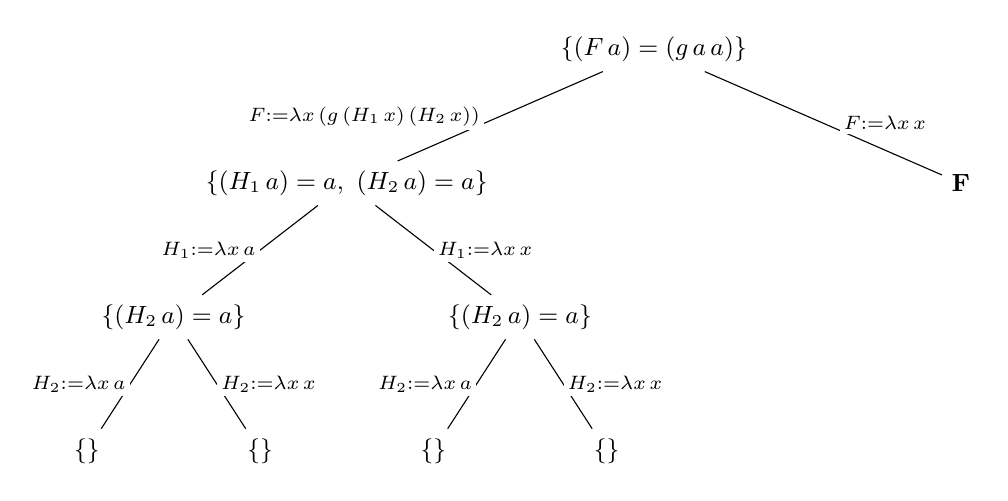
\begin{tikzpicture}[
  level distance=17mm,
  level 1/.style={sibling distance=78mm},
  level 2/.style={sibling distance=44mm},
  level 3/.style={sibling distance=22mm},
  every node/.style={font=\small},
  lab/.style={font=\scriptsize,inner sep=1.5pt,fill=white}]
\node {$\{(F\,a)=(g\,a\,a)\}$}
  child { node {$\{(H_1\,a)=a,\ (H_2\,a)=a\}$}
    child { node {$\{(H_2\,a)=a\}$}
      child { node {$\{\}$} edge from parent node[lab,left] {$H_2{:=}\lambda x\,a$} }
      child { node {$\{\}$} edge from parent node[lab,right] {$H_2{:=}\lambda x\,x$} }
      edge from parent node[lab,left] {$H_1{:=}\lambda x\,a$} }
    child { node {$\{(H_2\,a)=a\}$}
      child { node {$\{\}$} edge from parent node[lab,left] {$H_2{:=}\lambda x\,a$} }
      child { node {$\{\}$} edge from parent node[lab,right] {$H_2{:=}\lambda x\,x$} }
      edge from parent node[lab,right] {$H_1{:=}\lambda x\,x$} }
    edge from parent node[lab,left,xshift=-2mm] {$F{:=}\lambda x\,(g\,(H_1\,x)\,(H_2\,x))$} }
  child { node {$\mathbf{F}$}
    edge from parent node[lab,right,xshift=2mm] {$F{:=}\lambda x\,x$} };
\end{tikzpicture}
\caption{The matching tree for \mbox{$\forall a\,\forall g\,\exists F\,((F\,a)=(g\,a\,a))$}, after Figure~8.1 of the book
\book{219}. Arcs are labelled by substitutions; $\mathbf{F}$ marks a failure node; the four $\{\}$ leaves are
success nodes.}
\label{fig:hounif-tree}
\end{figure}

\begin{definition}[Matching tree {\book{219}}]\label{def:hounif-tree}
The \emph{matching tree} of a problem has as nodes the simplified matrices, viewed as multisets of equations
(the prefix is implicit), and as arcs the imitation and projection substitutions for one selected
flexible-rigid equation. Leaves are \emph{failure nodes}, \enquote{for which it is immediately apparent that there
are no solutions}, or \emph{success nodes}, whose matrix contains at most flexible-flexible equations. The
\emph{pre-unifier} of a success node is the composition of the arc labels on the path to it.
\end{definition}

\begin{theorem}[Completeness of matching trees {\book{219--220}}]\label{thm:hounif-tree}
If the problem at the root has a unifier, then the tree has a success node at a finite depth, and that unifier
is obtained by composing the pre-unifier of the success node with a unifier of the problem at that node. This
holds however the flexible-rigid equation to expand is chosen at each node.
\end{theorem}

So the choice of \emph{which equation} to work on is don't-care nondeterminism, while the choice of \emph{which
substitution} is don't-know nondeterminism. The bibliographic notes add that Huet's procedure, \enquote{which is
limited to determining unifiability, is nonredundant} \book{227}.

\subsection{Flexible-flexible equations and pre-unification}

Why stop at flexible-flexible equations? Because they always have a unifier, and their unifiers are
uncontrollable.

\begin{example}[A flexible-flexible residue {\book{217}}]\label{ex:hounif-residue}
With $a:i$ and $X,Y,g:i\to i$, take $\forall a\,\forall g\,\exists X\,\exists Y\,[(X\,a)=(g\,(Y\,a))]$. Imitation
$X:=\lambda x\,(g\,(H\,x))$ and simplification give $\forall a\,\forall g\,\exists H\,\exists Y\,[(H\,a)=(Y\,a)]$, which no
rule can reduce further. (The other alternative for $X$, the projection $X:=\lambda x\,x$, gives $a=(g\,(Y\,a))$,
a rigid-rigid clash.) The residue has the unifier $H,Y:=\lambda x\,a$ (making $X=\lambda x\,(g\,a)$), and many more: any
term built from $a$, $g$ and other existentials, abstracted over some of the occurrences of $a$, will do,
\enquote{too large and uncontrolled a set to try to generate explicitly} \book{218}.
\end{example}

\begin{proposition}[Canonical substitution {\book{217--218}}]\label{prop:hounif-canonical}
Associate with each primitive type $\tau$ a fixed new existential variable $H^\tau$, and with each type
$\tau_1\to\dots\to\tau_n\to\sigma$ ($\sigma$ primitive) the \emph{canonical constant term}
$\lambda x_1\dots\lambda x_n\,H^\sigma$. The \emph{canonical substitution} maps every existential variable of the
prefix to the canonical constant term of its type. For a problem with only flexible-flexible equations, the
canonical substitution is a unifier.
\end{proposition}

The reason is simple: under it both sides of every equation become $H^\beta$. For \cref{ex:hounif-residue}, with
$W$ the variable chosen for $i$, the canonical substitution is $\{\langle H,\lambda x\,W\rangle,\langle Y,\lambda x\,W\rangle\}$
\book{217}. Hence: \enquote{The reduction of a unification problem to a flexible-flexible form thus constitutes
success from the perspective of determining unifiability. The process of carrying out such a reduction is known
as \emph{pre-unification}, and the substitution that leads to the corresponding success is called a
\emph{pre-unifier}} \book{218}.

\subsection{Non-termination}

\begin{example}[An infinite branch with infinitely many answers {\book{218}}]\label{ex:hounif-loop}
Let $x:i$ and $g,F:i\to i$: $\forall g\,\exists F\,\forall x\,[(F\,(g\,x))=(g\,(F\,x))]$. The single projection
$F:=\lambda x\,x$ solves it. The imitation $F:=\lambda x\,(g\,(H\,x))$ followed by simplification gives
$\forall g\,\exists H\,\forall x\,[(H\,(g\,x))=(g\,(H\,x))]$: the same problem with $H$ in place of $F$. Repeating
forever, the paths of the tree yield $F:=\lambda x\,x,\ \lambda x\,(g\,x),\ \lambda x\,(g\,(g\,x)),\dots$
\end{example}

\begin{example}[An infinite branch and no answer {\book{220}}]\label{ex:hounif-noanswer}
Add a second equation, with constants $a,b:i$: $\forall g\,\exists F\,\forall x\,[((F\,(g\,x))=(g\,(F\,x)))\wedge(F\,a)=(F\,b)]$.
\enquote{The second equation in the matrix here causes each of the unifiers that we have seen for the first
equation to be rejected} \book{220}: $F=g^k$ gives $g^k\,a=g^k\,b$, a clash. The tree has no success node but has an
infinite path. As unifiability is undecidable, such problems must exist \book{220}.
\end{example}

\begin{kanren}[the matching tree is a miniKanren search tree]
Imitation versus projection is don't-know choice among at most $n+1$ alternatives, i.e.\ a disjunction; the
matching tree is the search tree of those disjunctions. A depth-first interpreter, like $\lambda$Prolog's, can be
trapped in the infinite imitation branch of \cref{ex:hounif-loop} before it ever tries the projection.
miniKanren's interleaving \scm{or°} instead reaches every success node at finite depth, provided each expansion
step is guarded by a suspension (as \scm{define-relation} and \scm{fresh°} provide). The fairness is
skewed: \scm{or°} nests the binary interleaving to the right, so with $k$ alternatives the first one gets
about half of the steps; and conjunction gives no fairness guarantee across an infinite first conjunct.
Two hard limits remain. First, \cref{ex:hounif-noanswer} makes even \scm{(run 1 ...)} diverge, and no search
strategy can fix that. Second, imitation and projection need types at run time, which \micro{} does not have.
A Huet layer is therefore at best an opt-in, typed search over equations that the deterministic core has set
aside; see \cref{sec:roadmap-later-huet} (and \cref{sec:design-space} for why Huet's search is not the meaning of \scm{=°}).
\end{kanren}

% ============================================================================================
\section{Higher-order patterns}\label{sec:hounif-llambda}

\Cref{ch:lambdatree} introduced $\Llam$ as a programming discipline. The book recalls it as follows.

\begin{definition}[The $\Llam$ condition {\book{220}}, {\cite{Miller1991}}]\label{def:hounif-llambda}
A program clause or goal formula $B$ is in $\Llam$ if all quantification in $B$ is over non-predicate types and
\enquote{every subterm of $B$ of the form $(x\,t_1\dots t_n)$ in which $x$ is an essentially existentially
quantified variable is such that $t_1,\dots,t_n$ are distinct variables that are universally quantified within
the scope of the quantifier binding $x$} \book{220}. Transposed to a unification problem: every flexible subterm
$(F\,t_1\dots t_n)$ has as arguments \emph{distinct} universal variables quantified \emph{to the right of $F$} in
the prefix. Such a term is a \emph{(higher-order) pattern}.
\end{definition}

The case $n=0$ is allowed, so a bare logic variable is a pattern, and first-order unification is a special
case. Miller's formal definition~\cite[Fig.~3, p.~10--11]{Miller1991} is a judgement $Q\vdash_0 t:\tau$ relative
to a prefix $Q$, whose key rule says that $x\,y_1\cdots y_n$ is well formed when \enquote{$x$ is existentially
quantified in $Q$ to the left of where the distinct variables $y_1\dots y_n$ are universally quantified}.
\Cref{tab:hounif-patterns} gives a feel for the definition.

\begin{table}[t]
\centering\small
\caption{Patterns and non-patterns among the chapter's examples.}
\label{tab:hounif-patterns}
\begin{tabular}{@{}lll@{}}
\toprule
problem & pattern? & why \\
\midrule
$\exists F\,\forall x\,\forall y\,[(F\,x\,y)=\dots]$ & yes & distinct universals, right of $F$ \\
$\forall a\,\exists F\,[(F\,a)=\dots]$ (\cref{ex:hounif-nomgu}) & no & $a$ is quantified \emph{outside} $F$ \\
$\exists F\,\forall x\,[(F\,x\,x)=x]$ & no & arguments not distinct \\
$\forall g\,\exists F\,\forall x\,[(F\,(g\,x))=\dots]$ (\cref{ex:hounif-loop}) & no & argument is not a variable \\
$\exists F\,\exists N\,[(F\,N)=\dots]$ (the \lp{subst} clause) & no & argument is existential \\
$\forall f\,\exists X\,[X=(f\,X)]$ & yes & $n=0$ \\
\bottomrule
\end{tabular}
\end{table}

\begin{example}[Discharging a constant {\cite[p.~4--5]{Miller1991}}]\label{ex:hounif-discharge}
Miller motivates the fragment with \lp{append}. With the program
\[
  \forall x\,\forall l\,\forall k\,\forall m\,(\mathit{append}\ l\ k\ m\imp\mathit{append}\ (\mathit{cons}\ x\ l)\ k\ (\mathit{cons}\ x\ m)),
  \qquad\forall k\,(\mathit{append}\ \mathit{nil}\ k\ k),
\]
try to find $X$ such that $\forall y\,(\mathit{append}\ (\mathit{cons}\ a\ (\mathit{cons}\ b\ \mathit{nil}))\ y\ X)$ is
provable. The $\forall y$ introduces a new constant $k$, and two backchaining steps succeed only if
$X$ is instantiated with $(\mathit{cons}\ a\ (\mathit{cons}\ b\ k))$, which is impossible because $X$ was chosen
before $k$ existed. \enquote{Such a failure here is quite sensible since the value of $X$ should be independent of the
choice of the constant used to instantiate $\forall y$}. Now ask instead for
$\forall y\,(\mathit{append}\ (\mathit{cons}\ a\ (\mathit{cons}\ b\ \mathit{nil}))\ y\ (H\,y))$. The same steps
produce the pattern equation
\[(H\,k)=(\mathit{cons}\ a\ (\mathit{cons}\ b\ k)).\]
Two $\lambda$-terms for $H$ make it true, $\lambda w\,(\mathit{cons}\ a\ (\mathit{cons}\ b\ k))$ and
$\lambda w\,(\mathit{cons}\ a\ (\mathit{cons}\ b\ w))$, but \enquote{since $H$ cannot contain $k$ free, only the second
of these possible substitutions will succeed}. Miller calls this \emph{discharging} the constant $k$ from the
term: $H$ is the computed answer with the choice of eigenvariable abstracted away. In terms of Huet's procedure: imitation of
$\mathit{cons}$, $a$, $\mathit{cons}$, $b$ is forced, and at the leaf $k$ only the projection is legal, because
imitating $k$ would violate the scope condition. The pattern algorithm below does this in one walk.
\end{example}

\begin{definition}[$\beta_0$ {\book{206}}]
$\beta_0$-conversion is the special case $(\lambda x\,s)\,x=s$ of $\beta$; with $\alpha$ it is equivalent to
$(\lambda y\,s)\,x=s[x/y]$, provided $x$ is not free in $\lambda y\,s$.
\end{definition}

Under the $\Llam$ condition, instantiating a logic variable only ever creates $\beta_0$-redexes: \enquote{simply
replacing the bound variables within the body of an abstraction with a new set of names} \book{220}. A
$\beta_0$-step makes the term smaller, so we may expect its inverse, $\Llam$-unification, to be much better
behaved than inverting full $\beta$ \book{220}.

\begin{pitfall}[$\beta_0$ alone is not enough]
$\Llam$ problems are unification problems modulo $\alpha,\beta_0,\eta$, but not conversely. The problem
$\forall x\,(F\,x\,x=x)$ needs only $\beta_0$, yet has the two incomparable unifiers $\lambda u\lambda v\,u$ and
$\lambda u\lambda v\,v$ \book{208}. The \emph{distinctness} of the arguments is what buys most general unifiers,
not merely the shape of the redexes.
\end{pitfall}

\subsection{Why the procedure becomes deterministic}

Raising preserves the $\Llam$ condition \book{208, 220--221}, so we may still assume a $\forall\bar a\,\exists\bar X\,\forall\bar y$
prefix, and rigid-rigid simplification \enquote{applies unchanged} \book{221}. The interesting case is
flexible-rigid.

\begin{lemma}[At most one useful substitution {\book{221}}]\label{lem:hounif-one}
Let $(F\,c_1\dots c_n)=(c\,t_1\dots t_m)$ with $F$ existential and $c_1,\dots,c_n$ distinct universals quantified
in the scope of $F$. Then at most one imitation or projection substitution avoids an immediate clash.
\end{lemma}
\begin{proof}[Argument]
If $F$ is in the scope of $c$ ($c$ is to the left of $F$, e.g.\ a signature constant), then $c$ differs from every
$c_i$, which are to the right of $F$; every projection produces a head $c_i\ne c$ and clashes, so only
imitation can succeed. If $c$ is in the scope of $F$, imitation is not allowed, and the $i$-th projection
succeeds only if $c_i=c$; since the $c_i$ are distinct, at most one $i$ qualifies, and if $c\notin\bar c$ the
equation fails. \enquote{The preceding observations can be built into the substitution selection process so as to
make it entirely deterministic} \book{221}.
\end{proof}

Moreover the class is preserved: the substitutions considered have the form
\[\lambda x_1\dots\lambda x_n\,(@\,(H_1\,x_1\dots x_n)\cdots(H_k\,x_1\dots x_n))\]
with $@$ either $c$ or some $x_i$ and the
$H_j$ quantified where $F$ was; substituted into $(F\,c_1\dots c_n)$ and $\beta_0$-reduced, it yields again
patterns $(H_j\,c_1\dots c_n)$ \book{221}.

\subsection{Flexible-flexible pattern equations have mgus}\label{sec:hounif-ff}

Here is the second change. In $\Llam$ a flexible-flexible equation has the form
\[(F\,c_1\dots c_n)=(G\,d_1\dots d_m),\]
with the $c_i$ and $d_j$ universals in the scope of $F$ and $G$, and in a $\forall\exists\forall$ prefix $F$ and $G$ are
\enquote{effectively bound \enquote{at the same place}} \book{222}.

\begin{proposition}[Flexible-flexible mgus {\book{222}}]\label{prop:hounif-ff}
Let $H$ be a new existential quantified at the place of $F$.
\begin{itemize}
  \item \textbf{Different heads} ($F\ne G$). Let $e_1,\dots,e_\ell$ list the variables common to $c_1,\dots,c_n$ and
    $d_1,\dots,d_m$. Then
    \[\{\langle F,\ \lambda c_1\dots\lambda c_n\,(H\,e_1\dots e_\ell)\rangle,\ \langle G,\ \lambda d_1\dots\lambda d_m\,(H\,e_1\dots e_\ell)\rangle\}\]
    is an mgu.
  \item \textbf{Same head} ($F=G$, so $n=m$). Let $e_1,\dots,e_\ell$ list the $c_i$ such that $c_i=d_i$.
    Then
    \[\{\langle F,\ \lambda c_1\dots\lambda c_n\,(H\,e_1\dots e_\ell)\rangle\}\]
    is an mgu.
\end{itemize}
\end{proposition}
In the first case a common instance $t$ cannot contain a $c_i$ that is not also among the $d_j$, and conversely;
every such $t$ is an instance of $(H\,\bar e)$. In the second case the \emph{same} substitution acts on both sides,
so a variable survives only if it sits in the \emph{same argument position} on both sides \book{222}. (The
binders reuse the names $c_i$, so in $\lambda c_1\dots\lambda c_n\,(H\,e_1\dots e_\ell)$ the $e$'s are bound.)

\begin{pitfall}[same head: positions, not sets]
For $\forall x\,\forall y\,[(F\,x\,y)=(F\,y\,x)]$ the arguments are the same \emph{set}, but no position agrees, so
$\ell=0$ and the mgu is $F:=\lambda x\lambda y\,H$. Intersecting sets, as in the different-heads case, would
wrongly keep both arguments.
\end{pitfall}

\begin{theorem}[Mgus for higher-order patterns {\book{222}}, {\cite{Miller1991}}]\label{thm:hounif-mgu-exist}
\enquote{By combining the completeness property of matching trees with the observations that there is at most one
productive path in the tree and that most general unifiers can be provided for flexible-flexible pairs in the
$\Llam$ setting, it follows that the higher-order pattern unification problem possesses the property of having
most general unifiers} \book{222}. For $\forall\exists\forall$ problems the mgu is unique up to renaming of
variables~\cite[Prop.~9.2]{Miller1991}.
\end{theorem}

\subsection{Termination needs the occurs-check}

The procedure so far may still loop, even on first-order problems. For $\forall f\,\exists X\,[X=(f\,X)]$ the only
useful substitution is the imitation $X:=(f\,H)$, which produces $\forall f\,\exists H\,[H=(f\,H)]$, \enquote{identical
to the one with which we started} \book{222}. In $\Llam$ such behaviour arises only when the flexible head
occurs in the rigid side; so \enquote{we can ensure termination for the unification procedure by adding an
\enquote{occurs-check} to the substitution-generation step} \book{223}. Note that in $\Llam$ every occurrence of $F$ in
the rigid side is fatal: since pattern arguments are variables, there is no flexible occurrence that a later
substitution could erase.

% ============================================================================================
\section{The pattern unification algorithm}\label{sec:hounif-algo}

The book's final step is to fuse the imitation and projection traversal with the occurs-check traversal into
\enquote{a larger, more efficient substitution generation operation} \book{223}, called \emph{variable elimination}
\enquote{because of its similarity to an operation of the same name discussed for first-order unification}
\book{223}. We now state the whole algorithm precisely. The rules restate the book's \S8.3 and Miller's
transitions~\cite[\S6, p.~14--16]{Miller1991}. Two things the book leaves implicit are made explicit here: binders
\emph{inside} terms, and the order of pruning.

\paragraph{Setting.} The prefix is $\forall\bar a\;\exists\bar X\;\forall\Gamma$, where $\bar a$ are the signature
constants and $\Gamma$ is the growing list of inner universals, or \emph{eigenvariables}. A state is a pair
$\langle E;\theta\rangle$ of a multiset of equations and the substitution computed so far. Equations are symmetric.
$\theta$ is applied eagerly, and terms are kept $\beta_0$-normal.

\begin{mathpar}
\inferrule{\langle\{\lambda x\,s=\lambda x\,t\}\uplus E;\theta\rangle}{\langle\{s[z/x]=t[z/x]\}\cup E;\theta\rangle}\;\rulename{Abs}
\and
\inferrule{\langle\{\lambda x\,s=t\}\uplus E;\theta\rangle}{\langle\{s[z/x]=(t\,z)\}\cup E;\theta\rangle}\;\rulename{Eta}
\\
\inferrule{\langle\{(h\,s_1\dots s_n)=(h\,t_1\dots t_n)\}\uplus E;\theta\rangle}{\langle\{s_1=t_1,\dots,s_n=t_n\}\cup E;\theta\rangle}\;\rulename{Dec}
\and
\inferrule{\langle\{(h\,\bar s)=(k\,\bar t)\}\uplus E;\theta\rangle}{\bot}\;\rulename{Clash}
\\
\inferrule{\langle\{(F\,\bar c)=t\}\uplus E;\theta\rangle}{\langle\rho'(\rho(E));\ \rho'\circ\rho\circ\theta\rangle}\;\rulename{Elim}
\and
\inferrule{\langle\{(F\,\bar c)=(G\,\bar d)\}\uplus E;\theta\rangle}{\langle\sigma(E);\ \sigma\circ\theta\rangle}\;\rulename{FlexFlex}
\end{mathpar}
Side conditions:
\begin{itemize}
  \item \rulename{Abs}, \rulename{Eta}: $z$ is a fresh eigenvariable appended to $\Gamma$; in \rulename{Eta}, $t$ is
    not an abstraction. This is step~4 of the normal form, applied on demand.
  \item \rulename{Dec}, \rulename{Clash}: $h,k$ are rigid heads (signature constants or eigenvariables) and $h\ne k$
    in \rulename{Clash}. Untyped, an arity mismatch for the same head is also a clash~\cite[\S9.3]{Miller1991}.
  \item \rulename{Elim}: $(F\,\bar c)$ is a pattern, $t$ is rigid, and the elimination
    $\mathcal E_{F,\bar c}(t)$ of \cref{def:hounif-elim} succeeds with result $t'$ and pruning substitution $\rho$;
    then $\rho'=\{\langle F,\lambda\bar c.\,t'\rangle\}$. If $\mathcal E$ fails, the state goes to $\bot$.
  \item \rulename{FlexFlex}: both sides are patterns and $\sigma$ is the mgu of \cref{prop:hounif-ff}; for the
    same head with all positions agreeing, the equation is simply deleted.
  \item A flexible term that is \emph{not} a pattern blocks the rules; we come back to it in
    \cref{sec:hounif-dynamic}.
\end{itemize}

\begin{definition}[Variable elimination]\label{def:hounif-elim}
Let $(F\,c_1\dots c_n)$ be a pattern. The elimination $\mathcal E_L(t)$ of a $\beta_0$-normal term $t$, relative to a
set $L$ of variables bound by $\lambda$s \emph{inside} $t$ (initially $L=\emptyset$), either fails or returns a term,
and may record pruning bindings in $\rho$. It is defined by cases on $t$, after applying the pruning bindings
recorded so far:
\[
\begin{array}{@{}l@{\quad}l@{\quad}l@{}}
  \mathcal E_L(a) &= a & a \text{ a signature constant (outer } \forall)\\
  \mathcal E_L(y) &= y & y\in\bar c\cup L\\
  \mathcal E_L(y) &= \text{fail (scope)} & y\in\Gamma\setminus(\bar c\cup L)\\
  \mathcal E_L(\lambda z\,s) &= \lambda z\,\mathcal E_{L\cup\{z\}}(s)\\
  \mathcal E_L(h\,s_1\dots s_k) &= \mathcal E_L(h)\,\mathcal E_L(s_1)\dots\mathcal E_L(s_k) & h \text{ rigid}\\
  \mathcal E_L(F\,\bar s) &= \text{fail (occurs)}\\
  \mathcal E_L(G\,d_1\dots d_m) &= G'\,e_1\dots e_\ell & G\ne F \text{ a pattern; see below}
\end{array}
\]
In the last case $e_1\dots e_\ell$ is the subsequence of $d_1\dots d_m$ of the variables in $\bar c\cup L$. If
$\ell=m$, nothing is pruned and $G'=G$. Otherwise the \emph{pruning substitution}
$\langle G,\ \lambda d_1\dots\lambda d_m\,(G'\,e_1\dots e_\ell)\rangle$, with $G'$ new and quantified at the place of $G$,
is added to $\rho$.
\end{definition}

This is the book's description \book{223}, case by case. \enquote{This pruning substitution replaces $G$ with the term
$\lambda d_1\dots\lambda d_m\,(G'\,e_1\dots e_\ell)$, where $G'$ is a new existentially quantified variable, and
$e_1,\dots,e_\ell$ is some listing of the variables that are common to $c_1,\dots,c_n$ and $d_1,\dots,d_m$. Now let the
result of applying these auxiliary substitutions to the term $t$ be $t'$. Then the main part of variable
elimination checks whether there are occurrences in $t'$ either of $F$ or of variables different from the ones in
$c_1,\dots,c_n$ that are quantified universally within the scope of the quantifier binding $F$. If there are such
occurrences, then it marks the problem as one for which no unifiers exist. Otherwise, it generates the
substitution $\lambda c_1\dots\lambda c_n\,t'$ for $F$ and replaces the equation under consideration by $\top$.}

Read the definition as an \emph{inversion}. $F$ applied to $\bar c$ must produce $t$, so $\lambda\bar c.\,t'$ must
\enquote{undo} the application: every $c_i$ in $t$ becomes the $i$-th bound variable of $F$'s binder. A universal
that $F$ cannot see and that $F$ does not receive as an argument has no preimage. In a rigid position it makes the
problem unsolvable; inside the arguments of another flexible term $G$ it can be removed by \emph{pruning}, that
is, by committing $G$ to ignore that argument. Imitation (rigid heads copied) and projection (a $c_i$ copied as a
bound variable) are both inside this single walk.

\begin{pitfall}[four things the prose leaves implicit]
\leavevmode
\begin{enumerate}[nosep]
  \item An out-of-scope universal is fatal only in a \emph{rigid} position. Inside the argument list of a
    flexible subterm it is pruned. The book's \cref{ex:hounif-8j} below says exactly this: \enquote{in a position that
    is not the argument of a flexible term} \book{224}.
  \item Variables bound by $\lambda$s \emph{inside} $t$ are always allowed, both in rigid positions and as kept
    arguments of pruned terms; this is the set $L$. The book never needs $L$ because its normal form has no inner
    binders at the top, but terms like $h\,(\lambda z\,(G\,z\,w))$ have them below the top.
  \item Pruning \emph{binds other variables} ($G$) as a side effect, although the equation is about $F$. If $G$
    occurs twice, the second occurrence must be examined \emph{after} the first pruning, which may prune again
    (\cref{ex:hounif-two}).
  \item Pruning never meets $F$ itself: that is the occurs failure.
\end{enumerate}
\end{pitfall}

\begin{theorem}[Pattern unification is unitary and terminating]\label{thm:hounif-mgu}
On a $\forall\exists\forall$ problem whose flexible subterms are all patterns, the rules terminate. If they reach $\bot$
the problem has no unifier; otherwise they end in $\langle\emptyset;\theta\rangle$ and $\theta$ is an mgu
(\book{222--224}; \cite[Thm.~7.1, Prop.~7.3]{Miller1991}).
\end{theorem}

Miller proves termination with a lexicographic measure: the number of existentials, the total size of the
equations, the number of equations, a weight of the universals, and the number of possibly prunable
occurrences~\cite[Thm.~7.1, p.~18]{Miller1991}. Intuitively, \rulename{Elim} and the different-heads case of
\rulename{FlexFlex} each remove one existential for good (a pruned $G$ is traded for one $G'$; $F$ and $G$ are
traded for one $H$); the same-head case trades $F$ for one $H$, so the number of existentials stays put, but the
equation disappears (both sides become $H\,\bar e$); and the other rules shrink the problem. The
occurs-check is what prevents the $X=(f\,X)$ loop. Qian later showed the problem can be solved in linear
time~\cite{Qian1996}.

Two remarks complete the picture. First, \enquote{types have no bearing on the shapes of unifiers}: the
algorithm \enquote{makes no use at all of type information in determining unifying substitutions}, though types are
still needed to guarantee correctness, for example that same-head flexible terms have equal arity \book{224}.
Miller's untyped variant replaces the type guarantee by two failures, an arity mismatch in \rulename{Dec} and
same-head flexible terms of different arity, and uses $\eta$-expansion \enquote{only on terms which, if typed, must
have functional type}~\cite[\S9.3]{Miller1991}. That is the variant an untyped Scheme host needs. Second, the
result is a genuine algorithm, as for first-order unification: \enquote{In both cases, term simplification and
variable elimination constitute the critical parts of the computation, although variable elimination has a more
involved structure in the higher-order pattern unification case} \book{224}.

% ============================================================================================
\section{Worked traces}\label{sec:hounif-traces}

Every result below was also checked mechanically with the Scheme transliteration of \cref{sec:hounif-nipkow}.
The book does not number its unification problems. We label them 8.A--8.M in their order of appearance in
the book's Chapter~8, as the proposal's test suite does, except 8.M, the problem $\forall x\,(F\,x\,x=x)$ of
\book{208} in the book's Chapter~7. The main example below is 8.H, the occurs and scope failures are 8.I
and 8.J, and the eager-versus-delayed raising of \cref{ex:hounif-8k} is 8.K.

\begin{example}[The book's main example {\book{223--224}}]\label{ex:hounif-8h}
With $x,y,w:i$, $f,g:i\to i$ and $U,V:i\to i\to i$, solve
\[
  \forall f\,\forall g\,\exists U\,\exists V\,\forall w\,\forall x\,\forall y\,[(f\,(U\,x\,y))=(f\,(g\,(V\,y\,w)))].
\]
\end{example}
\begin{tutorial}[the book's main example, step by step]
\begin{enumerate}
  \item Both sides are rigid with head $f$: \rulename{Dec} leaves $(U\,x\,y)=(g\,(V\,y\,w))$.
  \item The left side is the pattern $U$ applied to $\bar c=(x,y)$, and the right side is rigid: \rulename{Elim}.
    Walk $t=g\,(V\,y\,w)$ with $L=\emptyset$:
    \begin{itemize}[nosep]
      \item $g$ is a signature constant, so it is kept (this is the imitation part);
      \item $(V\,y\,w)$ is a flexible pattern with $\bar d=(y,w)$. Of these, $y\in\bar c$ is kept and $w\notin\bar c$ must
        go: prune $V:=\lambda y\,\lambda w\,(V'\,y)$, so the subterm becomes $(V'\,y)$.
    \end{itemize}
    Now $t'=g\,(V'\,y)$. $U$ does not occur in it, and its only inner universal $y$ is in $\bar c$, so bind
    $U:=\lambda x\,\lambda y\,(g\,(V'\,y))$.
  \item The matrix is empty. The mgu is $\{\langle V,\lambda y\lambda w\,(V'\,y)\rangle,\ \langle U,\lambda x\lambda y\,(g\,(V'\,y))\rangle\}$
    \book{224}.
\end{enumerate}
Check: $U\,x\,y\to_{\beta_0}g\,(V'\,y)$ and $V\,y\,w\to_{\beta_0}V'\,y$, so both sides become $f\,(g\,(V'\,y))$.
\end{tutorial}

\begin{example}[Occurs failure {\book{224}}]\label{ex:hounif-8i}
$\forall f\,\forall g\,\exists U\,\exists V\,\forall w\,\forall x\,\forall y\,[(U\,x\,y)=(g\,(U\,y\,w))]$: the walk meets
$(U\,y\,w)$, whose head is the variable being eliminated, so the problem fails, \enquote{because of the occurrence of
$U$, the head of the flexible term, in the rigid term}. Note that pruning cannot help: whatever $U$ does with its
arguments, the right side is one $g$ larger than the left.
\end{example}

\begin{example}[Scope failure {\book{224}}]\label{ex:hounif-8j}
$\forall f\,\forall g\,\exists U\,\exists V\,\forall w\,\forall x\,\forall y\,[(U\,x\,y)=(g\,w)]$ \enquote{has no unifiers
because the universally quantified variable $w$, which is not one of the arguments in $(U\,x\,y)$, appears on the
right-hand side of the equation and in a position that is not the argument of a flexible term}. Logically: $U$ is
chosen before $w$ and does not receive it, so it cannot produce it.
\end{example}

\begin{example}[Discharging, by elimination]
For \cref{ex:hounif-discharge}, $(H\,k)=(\mathit{cons}\ a\ (\mathit{cons}\ b\ k))$ with $\bar c=(k)$: the walk keeps the
signature constants $\mathit{cons}$, $a$, $b$ (imitation), meets $k\in\bar c$ and maps it to $H$'s bound variable
(projection), finds no flexible subterm to prune and no occurrence of $H$, and returns
$H:=\lambda w\,(\mathit{cons}\ a\ (\mathit{cons}\ b\ w))$, Miller's unique answer.
\end{example}

\begin{kanren}[the scope failure that surprised \texorpdfstring{$\lambda$}{λ}Kanren]
Ma and Friedman~\cite{MaFriedman2021} open with the miniKanren query
\texttt{(run 1 X (== (λ (a) X) (λ (b) b)))} and observe that it \enquote{fails. Under any existing higher-order
unification algorithm, X and a cannot be unified due to the scope restrictions}, while a novice expects
\texttt{X = a}. Read through \rulename{Abs}, the equation is $\exists X\,\forall z\,[X=z]$: \cref{ex:hounif-8j}
with $n=0$, so the failure is the \emph{correct} answer under the quantifier reading (no single $X$ equals every
$z$). Their proposal changes the semantics with de~Bruijn levels so that the query answers \texttt{(d0)};
\cref{ch:lkanren} examines that choice. Whichever semantics a new module picks, it must say so explicitly;
see \cref{ch:design}.
\end{kanren}

\begin{example}[Flexible-flexible, different heads]\label{ex:hounif-ffdiff}
For \cref{ex:hounif-ch4}, $\exists G\,\exists H\,\forall x\,\forall y\,[(G\,x)=(H\,y)]$: here $\bar c=(x)$ and
$\bar d=(y)$ have nothing in common, $\ell=0$, and \cref{prop:hounif-ff} gives
\[\{\langle G,\lambda x\,T\rangle,\ \langle H,\lambda y\,T\rangle\},\]
the book's \enquote{$\lambda w\,T$ for both} \book{113}. Had the
equation been $(G\,x\,y)=(H\,y)$, then $\bar e=(y)$ and the mgu would be $G:=\lambda x\lambda y\,(T\,y)$,
$H:=\lambda y\,(T\,y)$.
\end{example}

\begin{example}[Pruning under an inner binder]\label{ex:hounif-loc}
$\forall h\,\exists F\,\exists G\,\forall w\,\forall x\,[(F\,x)=(h\,(\lambda z\,(G\,z\,w)))]$. \rulename{Elim} with $\bar c=(x)$
walks $h$ (kept), then the abstraction, adding $z$ to $L$, then $(G\,z\,w)$: $z\in L$ is kept and $w$ is pruned,
$G:=\lambda z\lambda w\,(G'\,z)$. Result: $F:=\lambda x\,(h\,(\lambda z\,(G'\,z)))$. The local $z$ is legal everywhere below its
binder, which is item~2 of the pitfall after \cref{def:hounif-elim}.
\end{example}

\begin{example}[Two occurrences, two prunings]\label{ex:hounif-two}
$\forall g\,\exists F\,\exists G\,\forall w\,\forall x\,[(F\,x)=(g\,(G\,x\,w)\,(G\,w\,x))]$, with $\bar c=(x)$. The first
occurrence prunes the second argument: $G:=\lambda d_1\lambda d_2\,(G'\,d_1)$. The second occurrence now reads $(G'\,w)$,
and $w$ must be pruned again: $G':=\lambda d\,G''$. So $G:=\lambda d_1\lambda d_2\,G''$ and $F:=\lambda x\,(g\,G''\,G'')$. This
is correct: $G\,x\,w$ must not mention $w$, so $G$ ignores its second argument, and $G\,w\,x$ must not mention $w$,
so it ignores its first.
\end{example}

\begin{example}[$\eta$ on demand]
$\forall g\,\exists F\,[\lambda x\,(F\,x)=g]$: \rulename{Eta} gives $(F\,z)=(g\,z)$ with $z$ fresh, and \rulename{Elim}
binds $F:=\lambda z\,(g\,z)$, which is $\eta$-equal to $g$. Without \rulename{Eta}, an abstraction facing a constant
would be a spurious clash.
\end{example}

\begin{table}[t]
\centering\footnotesize
\caption{A test battery. The Huet column describes the pre-unification procedure exactly as the book presents it
in its \S8.2: it stops at flexible-flexible equations, and it has no occurs-check, since that is added only for
$\Llam$ \book{223}. The pattern column assumes the delaying discipline of \cref{sec:hounif-dynamic}.}
\label{tab:hounif-battery}
\begin{tabular}{@{}>{\raggedright\arraybackslash}p{0.29\textwidth}l>{\raggedright\arraybackslash}p{0.2\textwidth}>{\raggedright\arraybackslash}p{0.33\textwidth}@{}}
\toprule
problem (matrix) & $\Llam$? & pattern unification & Huet pre-unification \\
\midrule
$(F\,a)=(g\,a\,a)$ & no & not applicable (delay) & 4 answers \\
$(G\,x)=(H\,y)$ & yes & $G,H:=\lambda w\,T$ & already flex-flex; residue kept \\
$X=(f\,X)$ & yes & fail (occurs) & diverges (no occurs-check) \\
$(f\,(U\,x\,y))=(f\,(g\,(V\,y\,w)))$ & yes & mgu of \cref{ex:hounif-8h} & $U:=\lambda x\lambda y\,g\,(H\,x\,y)$, residue $(H\,x\,y)=(V\,y\,w)$ \\
$(U\,x\,y)=(g\,(U\,y\,w))$ & yes & fail (occurs) & diverges \\
$(U\,x\,y)=(g\,w)$ & yes & fail (scope) & fail \\
$(F\,(g\,x))=(g\,(F\,x))$ & no & delay & infinitely many answers \\
$(F\,x\,x)=x$ & no & delay & 2 answers \\
$(F\,x\,y)=(F\,y\,x)$ & yes & $F:=\lambda x\lambda y\,H$ & already flex-flex; residue kept \\
\bottomrule
\end{tabular}
\end{table}

% ============================================================================================
\section{Nipkow's de Bruijn algorithm}\label{sec:hounif-nipkow}

Nipkow~\cite{Nipkow1993} turned the transformation rules into \enquote{a directly executable functional program}
and then adapted it \enquote{to lambda-terms in de Bruijn's notation}, for typed and untyped terms alike. It is short and
complete, so we reconstruct it from the author's ML code.
It assumes a $\forall\exists\forall$ prefix, raised in a preprocessing phase \book{227}.

\paragraph{Encoding the prefix in the terms.} Existentials are global names \texttt{V F}, signature constants are
\texttt{C c}, and an abstraction \texttt{A t} has a body in which bound variables are de~Bruijn indices \texttt{B i}
(\cref{ch:lambdatree}). The inner $\forall$ block is not represented at all. To unify $\lambda w\lambda x\lambda y.\,s$ with
$\lambda w\lambda x\lambda y.\,t$, the algorithm simply strips the binders, which is rule \rulename{Abs}, and the
\emph{loose} indices of $s$ and $t$ then play the inner universals: under three binders, $y$ is \texttt{B 0}, $x$
is \texttt{B 1}, $w$ is \texttt{B 2}. Because every existential is quantified outside every inner universal, the
values bound to the \texttt{V}s are closed terms, and \enquote{fresh eigenvariable} costs nothing.

\paragraph{The algorithm} in pseudo-code; $S$ is a triangular substitution, i.e.\ an association list that is
walked rather than applied.
\begin{Verbatim}[fontsize=\footnotesize]
devar(S, s):                          ; β0 by renaming
  if s = (V F) b1..bk and S binds F to λ^k.body
  then devar(S, body with each bound index renamed to the matching b)  else s
unif(S, s, t):  s := devar(S, s);  t := devar(S, t);  case
  A s', A t'  → unif(S, s', t')                          ; Abs
  A s', t     → unif(S, s', (↑t) (B 0))                  ; Eta (and symmetric)
  F ȳ,  G z̄   → flexflex(F, ȳ, G, z̄, S)
  F ȳ,  t     → flexrigid(F, ȳ, t, S)                    ; (and symmetric)
  a s̄,  b t̄   → if a = b and |s̄| = |t̄| then fold unif over the pairs else FAIL
flexrigid(F, ȳ, t, S):
  if F occurs in t through S then FAIL                   ; occurs-check
  u := t with each loose index i replaced by the position
       of (B i) in ȳ counted from the right, or by •     ; inversion
  return proj(S + [F ↦ λ^|ȳ|. u], u)
proj(S, s):  case devar(S, s) of                         ; scope check and pruning
  A s'               → proj(S, s')
  (C c) s̄, (B i) s̄   → fold proj over s̄
  • s̄                → FAIL                              ; out of scope, rigid position
  (V G) b̄            → S + [G ↦ λ^|b̄|. H (positions of b̄ that are not •)],  H new
flexflex(F, ȳ, F, z̄, S):                                ; same head
  if ȳ = z̄ then S else S + [F ↦ λ^|ȳ|. H (positions i with y_i = z_i)]
flexflex(F, ī, G, j̄, S):                                ; different heads
  if ī ⊆ j̄ then S + [G ↦ λj̄. F ī]  elif j̄ ⊆ ī then S + [F ↦ λī. G j̄]
  else S + [F ↦ λī. H (ī ∩ j̄),  G ↦ λj̄. H (ī ∩ j̄)]
\end{Verbatim}

Compare it with the rules of \cref{sec:hounif-algo}.
\begin{itemize}
  \item \textbf{Inversion first, pruning second.} \texttt{flexrigid} binds $F$ to $\lambda^{|\bar y|}.u$ \emph{before}
    pruning, so $u$ may still contain markers \texttt{•} inside the arguments of other flexible terms. That is
    harmless: \texttt{proj} then binds each such $G$ to a term that drops those positions, and since $S$ is
    triangular, every later \texttt{devar} through $F$ also goes through $G$ and never sees a marker.
    (Nipkow's ML encodes the marker as the index \texttt{B(\textasciitilde 10000)}, which shifting keeps
    negative.)
  \item \textbf{One walk.} Imitation is the copying of \texttt{C} heads, projection the renaming of loose
    indices, the scope check the \texttt{•} in rigid position, and pruning the \texttt{V} case: this is the
    book's \enquote{variable elimination}. Inner binders need no set $L$: below \texttt{A}, indices that refer to
    local binders are never shifted into markers.
  \item \textbf{\texttt{devar} is $\beta_0$.} Arguments of a bound existential are indices, so
    \enquote{substituting} only renames indices; no shifting of arbitrary terms is needed.
  \item \textbf{An optimisation in \texttt{flexflex}.} If one argument list is contained in the other, one variable
    is bound directly to the other instead of introducing $H$; up to renaming, this is the mgu of
    \cref{prop:hounif-ff}.
  \item \textbf{No pattern test.} The code assumes its input is a pattern problem; a non-pattern argument would
    simply not be handled correctly. A dynamic-$\Llam$ implementation adds a test there and delays
    (\cref{sec:hounif-dynamic}).
\end{itemize}

\begin{tutorial}[\cref{ex:hounif-8h} in de Bruijn form]
Under the three binders $w,x,y$ the equation is $f\,(U\,1\,0)=f\,(g\,(V\,0\,2))$. \rulename{Dec} on $f$ leaves
$U\,1\,0=g\,(V\,0\,2)$. Here $\bar y=(1,0)$: index~$1$ (that is $x$) sits at position $1$ from the right, index~$0$
($y$) at position $0$, and index~$2$ ($w$) is absent. So $u=g\,(V\,0\,\text{•})$ and $U:=\lambda\lambda.\,g\,(V\,0\,\text{•})$.
\texttt{proj} meets $V\,0\,\text{•}$ and prunes: $V:=\lambda\lambda.\,H\,1$, i.e.\ $\lambda y\lambda w\,(H\,y)$. Walking $U$'s
binding through $S$ gives $\lambda x\lambda y\,(g\,(H\,y))$, the book's answer.
\end{tutorial}

\subsection{An executable transliteration}

The following plain Scheme is a line-by-line transliteration of the de~Bruijn ML code (file
\texttt{lics93-db.ML}). It is \emph{not} a proposal for the new module's interface (that is \cref{ch:design}); it is
here so that you can run, trace and modify the algorithm. Terms are tagged lists, failure escapes through a
continuation, and \scm{(OUT)} is the marker \texttt{•}.

\begin{scheme}[fontsize=\footnotesize]
(define (tag t) (car t))
(define (V n) (list 'V n))  (define (C n) (list 'C n))  (define (B i) (list 'B i))
(define (A t) (list 'A t))  (define ($ s t) (list '$ s t))  (define OUT '(OUT))
(define escape #f)
(define (fail) (escape 'fail))

(define (strip t)                       ; head and arguments of an application spine
  (let loop ((t t) (ts '()))
    (if (eq? (tag t) '$) (loop (cadr t) (cons (caddr t) ts)) (cons t ts))))
(define (apps h ts) (fold (λ (t h) ($ h t)) h ts))  ; foldl op $
(define (abs n t) (if (zero? n) t (abs (- n 1) (A t))))
(define (hnf n h ts) (abs n (apps h ts)))           ; λ^n. h ts

(define (mapbnd f t)                    ; f on the loose indices of t; #f gives OUT
  (let mpb ((d 0) (t t))
    (case (tag t)
      ((B) (let ((i (cadr t)))
             (if (< i d) t (let ((j (f (- i d)))) (if j (B (+ j d)) OUT)))))
      ((A) (A (mpb (+ d 1) (cadr t))))
      (($) ($ (mpb d (cadr t)) (mpb d (caddr t))))
      (else t))))
(define (incr t) (mapbnd add1 t))

(define (red s bs js)                   ; β0: (λ^k s) applied to indices renames them
  (if (and (eq? (tag s) 'A) (pair? bs) (memq (tag (car bs)) '(B OUT)))
      (red (cadr s) (cdr bs) (cons (and (eq? (tag (car bs)) 'B) (cadr (car bs))) js))
      (apps (mapbnd (λ (i) (list-ref js i)) s) bs)))

(define (devar S s)                     ; walk the head through the triangular S
  (let ((ht (strip s)))
    (cond ((and (eq? (tag (car ht)) 'V) (assoc (cadr (car ht)) S))
           => (λ (p) (devar S (red (cdr p) (cdr ht) '()))))
          (else s))))

(define (occ F S t)
  (let occ ((t t))
    (case (tag t)
      ((V) (or (equal? F (cadr t))
               (cond ((assoc (cadr t) S) => (λ (p) (occ (cdr p)))) (else #f))))
      (($) (or (occ (cadr t)) (occ (caddr t))))
      ((A) (occ (cadr t)))
      (else #f))))

(define counter 0)
(define (newV)
  (set! counter (add1 counter)) (V (string->symbol (format "H~a" counter))))

(define (pos p xs)                      ; indices (from the right) of the xs with p
  (let loop ((xs xs))
    (cond ((null? xs) '())
          ((p (car xs)) (cons (B (length (cdr xs))) (loop (cdr xs))))
          (else (loop (cdr xs))))))
(define (idx bs b)                      ; the index of b in the binder list bs, or #f
  (let loop ((bs bs))
    (cond ((null? bs) #f)
          ((equal? (car bs) b) (length (cdr bs)))
          (else (loop (cdr bs))))))

(define (proj S s)                      ; scope check + pruning, one walk over s
  (let* ((ht (strip (devar S s))) (h (car ht)) (ss (cdr ht)))
    (case (tag h)
      ((A) (proj S (cadr h)))
      ((C B) (fold (λ (t S) (proj S t)) S ss))
      ((OUT) (fail))                    ; out-of-scope universal, rigid position
      ((V) (let ((keep (pos (λ (b) (eq? (tag b) 'B)) ss)))
             (cons (cons (cadr h) (hnf (length ss) (newV) keep)) S))))))

(define (flexflex1 F ym zn S)           ; same head: keep the positions that agree
  (if (equal? ym zn) S
      (let ((keep (pos (λ (p) (equal? (car p) (cdr p))) (map cons ym zn))))
        (cons (cons F (hnf (length ym) (newV) keep)) S))))
(define (lam im G jn) (hnf (length im) G (map (λ (j) (B (idx im j))) jn)))
(define (subset? xs ys) (every (λ (x) (member x ys)) xs))
(define (flexflex2 F im G jn S)         ; different heads
  (cond ((subset? im jn) (cons (cons G (lam jn (V F) im)) S))
        ((subset? jn im) (cons (cons F (lam im (V G) jn)) S))
        (else (let ((kl (filter (λ (i) (member i jn)) im)) (H (newV)))
                (cons (cons F (lam im H kl)) (cons (cons G (lam jn H kl)) S))))))
(define (flexflex F ym G zn S)
  (if (equal? F G) (flexflex1 F ym zn S) (flexflex2 F ym G zn S)))

(define (flexrigid F im t S)            ; occurs check, inversion, then pruning
  (if (occ F S t) (fail)
      (let ((u (mapbnd (λ (i) (idx im (B i))) t)))
        (proj (cons (cons F (abs (length im) u)) S) u))))

(define (unif S s t)
  (let ((s (devar S s)) (t (devar S t)))
    (cond ((and (eq? (tag s) 'A) (eq? (tag t) 'A)) (unif S (cadr s) (cadr t)))
          ((eq? (tag s) 'A) (unif S (cadr s) ($ (incr t) (B 0))))     ; η on demand
          ((eq? (tag t) 'A) (unif S ($ (incr s) (B 0)) (cadr t)))
          (else (cases S s t)))))
(define (cases S s t)
  (let ((hs (strip s)) (ht (strip t)))
    (cond ((and (eq? (tag (car hs)) 'V) (eq? (tag (car ht)) 'V))
           (flexflex (cadr (car hs)) (cdr hs) (cadr (car ht)) (cdr ht) S))
          ((eq? (tag (car hs)) 'V) (flexrigid (cadr (car hs)) (cdr hs) t S))
          ((eq? (tag (car ht)) 'V) (flexrigid (cadr (car ht)) (cdr ht) s S))
          ((and (equal? (car hs) (car ht)) (= (length (cdr hs)) (length (cdr ht))))
           (fold (λ (a b S) (unif S a b)) S (cdr hs) (cdr ht)))
          (else (fail)))))
\end{scheme}

The test driver, a printer that applies $S$ and turns indices back into names (omitted here), and the
problems are in \texttt{writers/ch07-hounif/nipkow.scm}. For instance, \cref{ex:hounif-8h} is posed as
\begin{scheme}
(define f (C 'f)) (define g (C 'g)) (define h (C 'h))
(define (lam3 t) (A (A (A t))))     ; ∀w ∀x ∀y as three binders: y = 0, x = 1, w = 2
;; Example 8.H: ∀f∀g∃U∃V∀w∀x∀y [(f (U x y)) = (f (g (V y w)))]
(run "8.H  f (U x y) = f (g (V y w))" '(U V)
     (lam3 ($ f ($ ($ (V 'U) (B 1)) (B 0))))
     (lam3 ($ f ($ g ($ ($ (V 'V) (B 0)) (B 2))))))
\end{scheme}
and the whole battery prints, with \texttt{H1}, \texttt{H2} the fresh variables and \texttt{V1} standing for the
book's $V'$:
\begin{answers}
8.H  f (U x y) = f (g (V y w))
  U := λx1. λx2. g (H1 x2)
  V := λx1. λx2. H1 x1
8.I  U x y = g (U y w)
  no unifier
8.J  U x y = g w
  no unifier
4.5  λx λy (G x) = λx λy (H y)
  G := λx1. H1
  H := λx1. H1
ff   λx λy (F x y) = λx λy (F y x)
  F := λx1. λx2. H1
8.K  U x = f (V1 x y z)
  U := λx1. f (H1 x1)
  V1 := λx1. λx2. λx3. H1 x1
eta  λx (F x) = g
  F := λx1. g x1
dup  λx (F x) = λx (g x x)
  F := λx1. g x1 x1
loc  F x = h (λz (G z w))
  F := λx1. h (λx2. H1 x2)
  G := λx1. λx2. H1 x1
two  F x = g (G x w) (G w x)
  F := λx1. g H2 H2
  G := λx1. λx2. H2
\end{answers}
Every line agrees with the hand derivations: \cref{ex:hounif-8h,ex:hounif-8i,ex:hounif-8j,ex:hounif-ffdiff,ex:hounif-loc,ex:hounif-two},
the same-head pitfall, and the eagerly raised form of \cref{ex:hounif-8k} below.

\begin{kanren}[what first-order unification does with the same terms]
\micro{} can already store de~Bruijn terms as records, but its unifier treats an application of a logic
variable as a pair of slots. This sometimes gives the right answer by luck, sometimes an ill-scoped one, and
sometimes a wrong failure. With \scm{(define-record lam body)}, \scm{(define-record app rator rand)} and
\scm{(define-record dbi n)}:
\begin{scheme}
(show "X = (f X)"
      (°->list #f (fresh° (q) (=° q (list 'f q)))))
(show "λx (F x) = λx (g x)"
      (°->list #f (fresh° (f) (=° (make-lam (make-app f (make-dbi 0)))
                                  (make-lam (make-app 'g (make-dbi 0)))))))
(show "λx (F x) = λx (g x x)"
      (°->list #f (fresh° (f) (=° (make-lam (make-app f (make-dbi 0)))
                                  (make-lam (make-app (make-app 'g (make-dbi 0)) (make-dbi 0)))))))
(show "λx (F x) = λx (g x 7)"
      (°->list #f (fresh° (f) (=° (make-lam (make-app f (make-dbi 0)))
                                  (make-lam (make-app (make-app 'g (make-dbi 0)) 7))))))
\end{scheme}
\begin{answers}
;; X = (f X)
()
;; λx (F x) = λx (g x)
((λ () 'g))
;; λx (F x) = λx (g x x)
((λ () (make-record-instance 'app 'g (make-record-instance 'dbi 0))))
;; λx (F x) = λx (g x 7)
()
\end{answers}
The occurs-check case is already right. The second answer is right up to $\eta$. The third binds $F$ to
\enquote{$g$ applied to index $0$} \emph{outside} any binder: a dangling index, where the mgu is
$F:=\lambda y\,(g\,y\,y)$ (\texttt{dup} above). The fourth fails, where the mgu is $F:=\lambda y\,(g\,y\,7)$. A
higher-order extension must therefore recognise a flexible application and run \rulename{Elim} on it rather than
decomposing it structurally; see \cref{ch:design}.
\end{kanren}

% ============================================================================================
\section{Mixed prefixes, levels and delayed equations}\label{sec:hounif-pragmatics}

Everything so far assumed a $\forall\exists\forall$ prefix. Real proof search does not deliver one. Each
\lp{pi x\ G} adds a universal, and each backchaining step adds existentials \emph{after} it, giving prefixes such as
$\forall\exists\forall\exists\forall\dots$ \book{224}. Raising them eagerly \enquote{has to be performed dynamically},
may raise existentials \enquote{over long lists of universally quantified variables} (typical of the \lp{pi}-based
recursion of \cref{ch:lambdatree}), and \enquote{often can be redundant and may have to be undone by a pruning
substitution at a later point} \book{224}.

\begin{example}[Eager versus delayed raising {\book{224--225}}]\label{ex:hounif-8k}
Consider
\[\forall f\,\exists U\,\forall x\,\forall y\,\forall z\,\exists V\,[(U\,x)=(f\,V)].\]
\begin{itemize}
  \item \emph{Eagerly}, raise $V$ over $x,y,z$:
    \[\forall f\,\exists U\,\exists V'\,\forall x\,\forall y\,\forall z\,[(U\,x)=(f\,(V'\,x\,y\,z))].\]
    Variable elimination
    immediately prunes $V':=\lambda x\lambda y\lambda z\,(W\,x)$, giving $U:=\lambda x\,(f\,(W\,x))$, so two of the three raised
    arguments were wasted work.
  \item \emph{Delayed}: record that $U$ may be raised over $f$ and $V$ over $x,y,z,f$. When solving, \enquote{noting
    the presence of $x$ as an argument of the flexible term and the possibility of raising $V$ over $x$, we would
    replace $V$ with the term $(V'\,x)$, where $V'$ is a new variable quantified at the same place in the prefix as
    $U$ and would produce the unifying substitution $\lambda x\,(f\,(V'\,x))$ for $U$} \book{225}.
\end{itemize}
\end{example}

The lists of universals that each existential may depend on \enquote{are all initial segments of the sequence of
variables that are universally quantified in the prefix, \dots{} and this information can be maintained and used
efficiently by attaching numerical indices to the quantified variables} \book{225}. This idea has two
literature sources.

\paragraph{Universe indices for \texttt{pi} goals~\cite{NadathurJayaramanKwon1995}.} In a WAM-style interpreter for
first-order hereditary Harrop formulas, \enquote{each time a universal quantifier is encountered, a new constant must
be introduced, giving rise to the next universe in the hierarchy}: the universe index is incremented and the new
constant is tagged with it. A logic variable is tagged with the current index, meaning \enquote{that a term may be
substituted for the variable only if all the constants appearing in the term have a smaller or identical tag}
(p.~16). Binding $X^i:=t$ then requires (1)~the usual occurs-check; (2)~that $t$ contains no constant with tag
greater than $i$; and (3)~that, before binding, the tags of the variables of $t$ greater than $i$ be lowered to
$i$, \enquote{to prevent a later instantiation of these variables from violating the restrictions on instantiations
for $X$} (p.~16).

\begin{example}[Why tags must be lowered {\cite[p.~16]{NadathurJayaramanKwon1995}}]
Program $\forall z\,(q(z)\imp p(d(z)))$, goal $\exists x\,\forall y\,(q(y)\imp p(x))$. After the quantifiers the goal
is $q(c^2)\imp p(X^1)$. Backchaining on the clause with a new $Z^2$ unifies $p(d(Z^2))$ with $p(X^1)$; binding
$X:=d(Z)$ lowers $Z$ to $Z^1$. The remaining goal $q(Z^1)$ must be matched against the hypothesis $q(c^2)$ and
\emph{fails}, because $c$ has tag $2>1$. Without step~(3), $Z$ would be bound to $c$ and $X$ would end up as
$d(c)$, mentioning a constant introduced after $X$.
\end{example}

\paragraph{Prefix erasure for patterns~\cite{NadathurLinnell2005}.} Nadathur and Linnell tag every variable $y$ with
$l(y)$, \enquote{the number of times an existential quantifier is immediately followed by a universal one in the prefix
up to and including the quantifier binding that occurrence}. Then \enquote{a universal variable $u$ is quantified
within the scope of the quantifier for an existential variable $x$ just in case $l(x)<l(u)$} (p.~8), so the pattern
test becomes local. Raising is restricted to what is needed: for $f(\bar y)=g(\bar z)$ with $l(f)\le l(g)$, $g$ needs
to be raised only over $\bar y{\Uparrow}g=\{u\in\bar y\mid l(u)\le l(g)\}$, the universals among $f$'s arguments that
$g$ may depend on. A combined rule (9$'$) binds $f$ and $g$ to a common new $h$ with $l(h)=l(f)$, applied first to
those universals and then to the common arguments (p.~9). Their Theorem~2 states that prefix erasure preserves
termination and mgus (p.~10), and their Figure~2 gives the single-traversal \texttt{mksubst}/\texttt{bnd} that
computes the binding, the pruning and the raising together (p.~11). The algorithm is used in Bedwyr, Abella and
Teyjus~2 \book{228}.

\paragraph{Variable elimination with levels.} Combining the two, \cref{def:hounif-elim} generalises to tagged
variables. This is our reconstruction, checked by hand on \cref{ex:hounif-8h,ex:hounif-8k}; Nadathur and Linnell's
Figure~2 is the authoritative version. Write $l(\cdot)$ for levels, with signature constants at the lowest level.
To eliminate $F$ in $(F\,\bar c)=t$, where pattern means that the $c_i$ are distinct universals with
$l(c_i)>l(F)$:
\begin{itemize}
  \item a universal $u$ in rigid position is kept if $u\in\bar c\cup L$ or $l(u)\le l(F)$ (since $F$ may mention it
    directly), and fails otherwise;
  \item a flexible pattern $(G\,\bar d)$ keeps the $d_j\in\bar c\cup L$ and the $d_j$ with $l(d_j)\le l(F)$, prunes the rest,
    and, if $l(G)>l(F)$, is \emph{also raised} over the $c_i$ with $l(c_i)\le l(G)$ that it does not already receive;
    the new $G'$ gets level $l(F)$. In \cref{ex:hounif-8k}, $l(U)=0$ and $l(x)=l(V)=1$, so $V$ (no arguments) is
    raised over $x$: $V:=(V'\,x)$ with $l(V')=0$, and $U:=\lambda x\,(f\,(V'\,x))$, as in the book;
  \item when no $c_i$ qualifies, raising degenerates to \emph{lowering}: $G:=\lambda\bar d.\,(G'\,\bar e)$ with
    $l(G')=l(F)$ and nothing added, which is step~(3) of the universe-index discipline above.
\end{itemize}

\paragraph{De Bruijn levels in ELPI~\cite{DunchevEtAl2015}.} ELPI makes the two notions of level coincide.
\enquote{When a clause's head is unified with the goal in a context of length $n$, the universally quantified variables
of the clause are instantiated to unification variables $X^n$ where the level $n$ records that $X$ has only
visibility of the initial prefix of length $n$ of the context. If later a fresh constant is added by the
\texttt{pi} rule, the constant occupies position $n+1$ \dots{} and it will not be allowed to occur in instances of the
variable $X^n$} (p.~4). Lowering a level is done by pruning: \enquote{unifying $B_0$ with $(\mathit{arr}\ C_1\ D_1)$
prunes $C$ and $D$ to level $0$} (p.~7), i.e.\ the higher-level variable is bound to a fresh lower-level one.

\begin{kanren}[levels and \micro]
\micro{} already allocates variables from a monotone counter, \scm{vars-count}, so creation order is a
linearisation of the dynamically built prefix. If eigenvariables were allocated from the same counter, the
creation index would give every variable its initial level for free. Three facts of the current engine matter for
any level discipline.
\begin{enumerate}[nosep]
  \item \emph{Level is not index.} Pruning and raising create a \emph{new} variable \enquote{quantified at the same
    place} as an \emph{old} one \book{225}, so a variable's level must be stored separately from its index.
  \item \emph{Orientation of var-var bindings.} Today the older variable is bound to the newer one. With scopes,
    binding a low-level $X$ to a high-level $Y$ lets a later binding of $Y$ smuggle a young eigenvariable into $X$.
    Either the orientation must follow levels, or the binding must lower $Y$, as in step~(3) above.
  \item \emph{Unification allocates.} Pruning, raising and the flexible-flexible $H$ create variables, so the
    unifier must return an updated \scm{vars-count}, and the bindings it reports must include the prunings of
    \emph{other} variables (item~3 of the pitfall after \cref{def:hounif-elim}), because constraint re-verification keys on them.
\end{enumerate}
How these requirements are met is the subject of \cref{ch:design}.
\end{kanren}

\subsection{Dynamic \texorpdfstring{$\Llam$}{Lλ}: delay what is not a pattern}\label{sec:hounif-dynamic}

A static $\Llam$ restriction \enquote{can rule out some useful programming idioms} \book{225}, the standard one
being substitution by meta-level $\beta$-reduction:
\begin{lprolog}
type   subst   (tm -> tm) -> tm -> tm -> o.
subst R N (R N).
\end{lprolog}
Here \lp{R} and \lp{N} are essentially existential, so \lp{(R N)} is not a pattern. \enquote{A common practical
resolution to this dilemma is to not impose the $\Llam$ restriction on program clauses statically but rather to
expect the condition to be satisfied by the unification problems that are encountered dynamically} \book{225--226}:
when \lp{subst} is called, \lp{R} and \lp{N} are expected to be instantiated, and \lp{(R N)} is then just a $\beta$-redex
to reduce. More generally: \enquote{we would treat any unification problem as if it is a higher-order
pattern-unification one. In the course of such a treatment, we might discover that a particular equation does not
respect the $\Llam$ condition. In this case, we might defer further consideration of this equation until such time
that substitutions resulting from solving other parts of the problem have altered its status} \book{226}.

The literature agrees on this design.
\begin{itemize}
  \item Dowek, Hardin, Kirchner and Pfenning~\cite{DowekHardinKirchnerPfenning1996}, \S5.4 (p.~13): equations outside
    the pattern fragment \enquote{should be postponed as constraints in the hope that they will be instantiated
    further}, which \enquote{avoids all branching during constraint simplification}. Their motivation is
    empirical~\cite{MichaylovPfenning1992}: the static restriction is too severe, but \enquote{almost all dynamically
    arising equations fall within the pattern fragment} (p.~2). Their algorithm phrases \rulename{Elim} as the
    inversion of a pattern substitution: $X[s]=b$ is solved by $X=b[s^{-1}]$ when every index of $b$ occurs in $s$
    (Prop.~8), with pruning computed together with the inverse (p.~11--12).
  \item Nadathur and Linnell~\cite{NadathurLinnell2005}, \S6: a non-pattern subterm met inside \texttt{bnd} can be
    replaced by a fresh flexible term, with the equation between them \emph{deferred}.
  \item Systems: Teyjus~1~\cite{NadathurMitchell1999} implemented (pre-)unification for unrestricted terms, while
    Teyjus~2 \enquote{only implements $\Llam$ unification}; Twelf and Minlog also implement only $\Llam$ unification,
    over an unrestricted term language \book{228}. ELPI's default for a problem outside the fragment is an error,
    with a deprecated option to delay it \enquote{for Teyjus compatibility}; its supported mechanism for suspension
    is instead a general syntactic constraint on goals, resumed when a variable is assigned.
\end{itemize}
Going the other way, \lp{subst} can be written inside $\Llam$ by making the object signature explicit with
\lp{copy} clauses (\cref{ch:lambdatree}), and by extension \enquote{it also may be possible to describe general
higher-order unification as a logic program in the $\Llam$ language} \book{226}~\cite{Miller1991}.

\begin{pitfall}[unifier versus solution; delayed is not solved]
A state with suspended equations has succeeded only \emph{conditionally}: its answer is a pre-unifier together
with residual constraints, and those must be printed with it. The canonical substitution of
\cref{prop:hounif-canonical} would make flexible-flexible residues \enquote{true}, but it introduces new existentials
$H^\tau$: it is a unifier, not a solution, and in a typed setting with an empty type there may be no closed solution
at all \book{211}. Untyped Scheme terms avoid that last problem~\cite[\S9.3]{Miller1991}, but not the first.
\end{pitfall}

\begin{kanren}[what delaying asks of a miniKanren]
Following the book's \enquote{defer further consideration} \book{226}, an \micro{}-style engine needs: a
place in the state for suspended equations; a wake-up step after each successful unification that retries the
suspended equations mentioning a variable just bound (the same \enquote{touched variables} mechanism that already
re-verifies disequalities); and reification that prints what is still suspended. Soft-cut, projection and
disequality must be audited, because each of them can observe a state whose success is only conditional.
Disequality needs care even without delays: the mgu of a pattern problem may contain \emph{new} variables
(pruning, the flexible-flexible $H$), and in $\neg\exists H.(X=\lambda x\,H)$ these are existentially quantified
inside the negation (equivalently, universally outside it), which a store of plain bindings would get wrong
(\cref{def:module-trial}). The concrete design is in \cref{ch:design}.
\end{kanren}

% ============================================================================================
\section{Summary}\label{sec:hounif-summary}

\begin{itemize}
  \item A unification problem is a quantified formula; its prefix decides who may depend on whom. The book
    normalises to a $\forall\exists\forall$ prefix by raising, to $\beta$-normal terms, to equal binders by $\eta$, and turns
    top binders into inner universals \book{212}.
  \item General higher-order unification has no mgus, may need infinite complete sets of unifiers, and is
    undecidable \book{213--214}.
  \item Huet's procedure: \rulename{Dec}/\rulename{Clash} on rigid-rigid pairs, imitation (scope-sensitive) or
    projection (type-sensitive) on flexible-rigid ones, success when only flexible-flexible equations remain
    (pre-unification; the canonical substitution unifies them). Its matching tree is complete but may have infinite
    branches, with or without answers \book{214--220}.
  \item In $\Llam$, flexible terms are patterns $F\,\bar c$ with distinct universals bound inside $F$'s scope. Only
    $\beta_0$ arises, at most one imitation or projection is useful, flexible-flexible pairs have explicit mgus
    (common arguments for different heads, agreeing positions for the same head), and with an occurs-check the
    procedure terminates: pattern unification is decidable and unitary \book{220--224}, \cite{Miller1991}.
  \item Variable elimination in one walk: keep rigid heads, map each $c_i$ to $F$'s $i$-th bound variable, keep local
    binders, prune the arguments of other flexible terms that $F$ cannot see, and fail on $F$ itself (occurs) or on an
    unseeable universal in rigid position (scope). Then $F:=\lambda\bar c.\,t'$ \book{223}.
  \item Nipkow's de Bruijn version is short (our Scheme transliteration of its core is under a hundred lines); loose indices are the inner universals, \texttt{devar}
    is $\beta_0$ by renaming, and inversion uses a marker that pruning removes \cite{Nipkow1993}. No types are needed
    \book{224}.
  \item In practice prefixes are mixed and dynamic: replace raising by levels on variables and eigenvariables,
    lower levels when binding, raise lazily only over the arguments needed \book{225},
    \cite{NadathurJayaramanKwon1995,NadathurLinnell2005,DunchevEtAl2015}.
  \item Dynamic $\Llam$: treat every equation as a pattern problem and \emph{delay} the non-patterns until bindings
    make them patterns; report what remains as residual constraints \book{226},
    \cite{DowekHardinKirchnerPfenning1996}.
  \item For \micro{}: first-order unification is the $n=0$ case; the extension needs eigenvariables, binders,
    flexible applications, levels, allocation inside unification, and a store of delayed equations; see
    \cref{ch:design}.
\end{itemize}
